\documentclass[12pt]{article}

\title{Activity 12: Arrays of Objects}
\author{Chris Mayfield}
\date{Spring 2018}

%\ProvidesPackage{cspogil}

% fonts
\usepackage[utf8]{inputenc}
\usepackage[T1]{fontenc}
\usepackage{mathpazo}

% spacing
\usepackage[margin=2cm]{geometry}
\renewcommand{\arraystretch}{1.4}
\setlength{\parindent}{0pt}

% orphans and widows
\clubpenalty=10000
\widowpenalty=10000
\pagestyle{empty}

% figures and tables
\usepackage{graphicx}
\usepackage{multicol}
\usepackage{tabularx}
\usepackage{wrapfig}

% fixed-width columns
\usepackage{array}
\newcolumntype{L}[1]{>{\raggedright\let\newline\\\arraybackslash\hspace{0pt}}m{#1}}
\newcolumntype{C}[1]{>{\centering\let\newline\\\arraybackslash\hspace{0pt}}m{#1}}
\newcolumntype{R}[1]{>{\raggedleft\let\newline\\\arraybackslash\hspace{0pt}}m{#1}}

% include paths
\makeatletter
\def\input@path{{Models/}{../../Models/}}
\graphicspath{{Models/}{../../Models/}}
\makeatother

% colors
\usepackage[svgnames,table]{xcolor}
\definecolor{bgcolor}{HTML}{FAFAFA}
\definecolor{comment}{HTML}{007C00}
\definecolor{keyword}{HTML}{0000FF}
\definecolor{strings}{HTML}{B20000}

% table headers
\newcommand{\tr}{\bf\cellcolor{Yellow!10}}

% syntax highlighting
\usepackage{textcomp}
\usepackage{listings}
\lstset{
    basicstyle=\ttfamily\color{black},
    backgroundcolor=\color{bgcolor},
    numberstyle=\scriptsize\color{comment},
    commentstyle=\color{comment},
    keywordstyle=\color{keyword},
    stringstyle=\color{strings},
    columns=fullflexible,
    keepspaces=true,
    showlines=true,
    showstringspaces=false,
    upquote=true
}

% code environments
\newcommand{\java}[1]{\lstinline[language=java]{#1}}%[
\lstnewenvironment{javalst}{\lstset{language=java,backgroundcolor=}}{}
\lstnewenvironment{javabox}{\lstset{language=java,frame=single,numbers=left}\quote}{\endquote}

% PDF properties
\usepackage[pdftex]{hyperref}
\urlstyle{same}
\makeatletter
\hypersetup{
  pdftitle={\@title},
  pdfauthor={\@author},
  pdfsubject={\@date},
  pdfkeywords={},
  bookmarksopen=false,
  colorlinks=true,
  citecolor=black,
  filecolor=black,
  linkcolor=black,
  urlcolor=blue
}
\makeatother

% titles
\makeatletter
\renewcommand{\maketitle}{\begin{center}\LARGE\@title\end{center}}
\makeatother

% boxes [optional height]
\newcommand{\emptybox}[1][10em]{
\vspace{1em}
\begin{tabularx}{\linewidth}{|X|}
\hline\\[#1]\hline
\end{tabularx}}

% models
\newcommand{\model}[1]{\section{#1}\nopagebreak}
\renewcommand{\thesection}{Model~\arabic{section}}

% questions
\newcommand{\quest}[1]{\subsection*{Questions~ (#1)}}
\newcounter{question}
\newcommand{\Q}{\vspace{1em}\refstepcounter{question}\arabic{question}.~ }
\renewcommand{\thequestion}{\#\arabic{question}}

% sub-question lists
\usepackage{enumitem}
\setenumerate[1]{label=\alph*)}
\setlist{itemsep=1em,after=\vspace{1ex}}

% inline answers
\definecolor{answers}{HTML}{C0C0C0}
\newcommand{\ans}[1]{%
\ifdefined\Student
    \leavevmode\phantom{~~\textcolor{answers}{#1}}
\else
    ~~\textcolor{answers}{#1}
\fi}

% longer answers [optional height]
\newsavebox{\ansbox}
\newenvironment{answer}[1][4em]{
\nopagebreak
\begin{lrbox}{\ansbox}
\begin{minipage}[t][#1]{\linewidth}
\color{answers}
}{
\end{minipage}
\end{lrbox}
\ifdefined\Student
    \phantom{\usebox{\ansbox}}%
\else
    \usebox{\ansbox}%
\fi}


\begin{document}

\maketitle

With arrays and objects, you can represent pretty much any type of data.
It's not only possible to have arrays of objects, but also objects of arrays, objects of objects, arrays of arrays, arrays of objects of arrays, and so forth.

\guide{
  \item Explain the differences when instantiating an array and an object.
  \item Rewrite a for loop (over an array) using an enhanced for loop.
  \item Use enhanced for loops to construct and search arrays of objects.
}{
  \item Developing algorithms for constructing and searching arrays. (Problem Solving)
}{
The first two objectives apply to \ref{hand-of-cards.tex}.
Students should understand the differences in syntax (i.e., using square brackets vs parentheses) as well as what happens behind the scenes (i.e., \texttt{new} invokes a constructor for objects but not arrays).

Keep an eye on what students write down for \ref{random}.
If their answer is superficial, challenge them to be more specific.
Report out on \ref{foreach}, and ask students why \java{i} is not an appropriate variable name for this loop (\java{i} typically stands for index or iteration).

This activity makes use of a simple Card class.
Be sure to take a look at the \github{CS1/Act12/Card.java}{source code} before facilitating.
It stores both the rank and suit as integers, and it does not perform any validation.
\ref{cnstr} in \ref{deck-of-cards.tex} asks students to implement a simple default value replacement.
This question can optionally be extended by having students call a setter method instead.

\ref{build} and \ref{search} are the most important questions.
Make sure students have enough time to develop the algorithms, and if possible, write the complete source code.
Consider reporting out after \ref{build} to bring the class back in sync, since there is so much time allocated for \ref{deck-of-cards.tex}.
}

\model{Hand of Cards}

Creating an array of objects is typically a 3-step process:

\begin{center}
\begin{minipage}[t]{155pt}

1. Declare the array \\[1ex]
\java{Card[] hand;}

\end{minipage}
\begin{minipage}[t]{155pt}

2. Instantiate the array \\[1ex]
\java{hand = new Card[5];}

\end{minipage}
\begin{minipage}[t]{155pt}

3. Instantiate each object \\[1ex]
\java{hand[0] = new Card(4, 2);}
\java{hand[1] = new Card(3, 1);}

\end{minipage}
\end{center}

\begin{center}
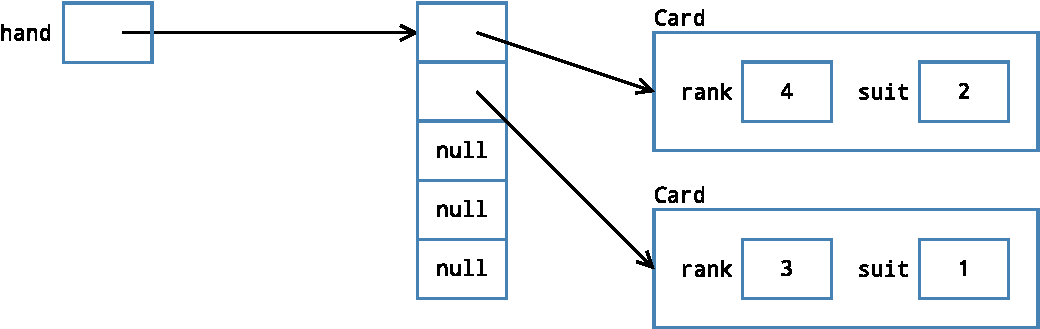
\includegraphics[width=465pt]{cards-array.pdf}
\end{center}


\quest{20 min}


\Q What is the type of the local variable \java{hand}?
What is the value of \java{hand} \emph{before} step 2?
What is the value of \java{hand} \emph{after} step 2?

\begin{answer}
The variable \java{hand} is an array of \java{Card} objects.
Before step 2, it's uninitialized (i.e., you can't read its value).
After step 2, its value is the memory location of the first array element.
\end{answer}


\Q When you create an array (e.g., ~\java{new Card[5]}) what is the initial value of each element?

\begin{answer}
The initial values are automatically set to null (for reference types). For arrays of integers, it's 0; for doubles, it's 0.0; for booleans, it's {\tt false}; for characters, it's the unicode character \chr{\textbackslash u0000}.
\end{answer}


\Q When you construct a new object (e.g., ~\java{new Card(4, 2)}) what are the initial values of its attributes (e.g., ~\java{this.rank})?

\begin{answer}
It depends on the constructor. For the \java{Card} class, the attributes \java{rank} and \java{suit} are initialized from the parameters. If there is no constructor, Java automatically initializes attributes to zero.
\end{answer}


\comment{The \java{new} operator requests a memory location to store an array or object.
Java automatically determines how much memory is needed and initializes the contents of the corresponding memory cells to zero.
That's why array elements and object attributes have default values, whereas local variables (not allocated with \java{new}) must be initialized before they are used.}


\Q \label{random}
Describe in your own words what the following statement does. Be sure to explain how the random part works.

\begin{center}
\java{hand[(int) (Math.random() * hand.length)] = null;}
\end{center}

\begin{answer}
\java{Math.random()} returns a value in the range [0, 1).
Multiplying that value by \java{hand.length} and then casting it to an integer gives a value in the range 0..5 inclusive.
So this statement randomly sets one of the \java{Card} references to {\tt null}.
\end{answer}


\Q \label{forcard}
What is the result of running the loop below?
What is the purpose of the nested if-statement?

\begin{javalst}
for (int i = 0; i < hand.length; i++) {
    if (hand[i] != null) {
        int suit = hand[i].getSuit();
        System.out.println("The suit of #" + i + " is " + Card.SUITS[suit]);
    }
}
\end{javalst}
\vspace{-1ex}

\begin{answer}
The loop prints the suits of all cards in the hand.
Because some of the cards are {\tt null}, the if-statement prevents {\tt NullPointerException}.
\end{answer}


\Q The \textit{enhanced for loop} allows you to iterate the elements of an array.
Another name for this structure is the ``for each'' loop.
Rewrite the following example using a standard for loop.

\vspace{1ex}
\begin{javalst}
String[] days = {"Sun", "Mon", "Tue", "Wed", "Thu", "Fri", "Sat"};
for (String day : days) {
    System.out.println(day + " is a great day!");
}
\end{javalst}
\vspace{-1em}

\begin{answer}[5em]
\begin{javaans}
for (int i = 0; i < days.length; i++) {
    System.out.println(days[i] + " is a great day!");
}
\end{javaans}
\end{answer}


\Q In contrast to enhanced for loops, what does a standard for loop typically iterate?
Why would it be misleading to name the enhanced for loop variable \java{i} instead of \java{day}?

\begin{answer}[3em]
Standard for loops typically iterate indexes; that's why the variable is almost always named \java{i}.
\end{answer}


\Q \label{foreach}
Rewrite the loop in \ref{forcard} using an enhanced for loop.
Use an appropriate variable name for the \java{Card} object (i.e., not \java{i}).
For simplicity, you may omit the \java{System.out.println} line.

\vspace{-1ex}
\begin{answer}[7em]
\begin{javaans}
for (Card card : hand) {
    if (card != null) {
        int suit = card.getSuit();
    }
}
\end{javaans}
\end{answer}

\model{Deck of Cards}

There are 52 cards in a standard deck.
Each card belongs to one of four suits (Clubs, Spades, Hearts, and Diamonds) and one of 13 ranks (Ace, 2, 3, 4, 5, 6, 7, 8, 9, 10, Jack, Queen, and King).
The array below is one-dimensional, but the cards are displayed on four lines for convenience.

\begin{center}
% http://www.milefoot.com/math/discrete/counting/cardfreq.htm
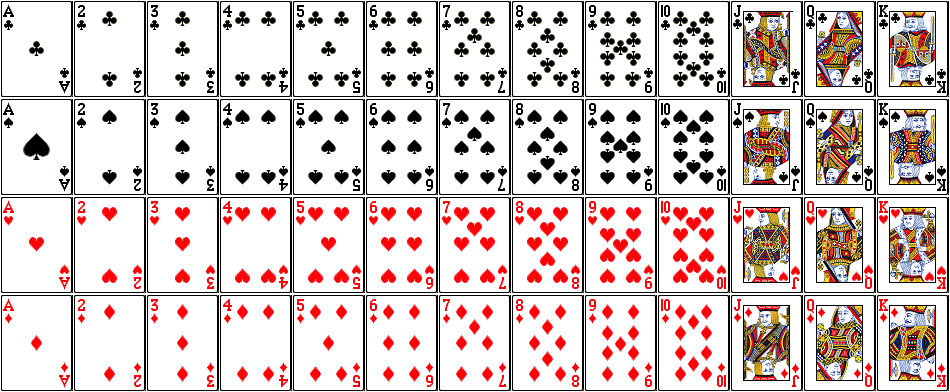
\includegraphics[width=\linewidth]{playing-cards1.png}
\end{center}


\quest{25 min}


\Q \label{cnstr}
Implement the following constructor.
The class has two attributes: \java{rank} and \java{suit}.
%You may assume the arguments are valid (rank is between 1 and 13, and suit is one of the four strings).
Make sure the arguments are within range, and if not, replace them with the minimum value.

\begin{javalst}
/**
 * Constructs a face card given its rank and suit.
 *
 * @param rank face value (1 = ace, 11 = jack, 12 = queen, 13 = king)
 * @param suit category (0 = clubs, 1 = diamonds, 2 = hearts, 3 = spades)
 */
public Card(int rank, int suit) {
\end{javalst}

\vspace*{-1em}
\begin{answer}[14em]
\begin{javaans}
    if (rank < 1 || rank > 13) {
        this.rank = 1;
    } else {
        this.rank = rank;
    }

    if (suit < 0 || suit > 3} {
        this.suit = 0;
    } else {
        this.suit = suit;
    }
\end{javaans}
\end{answer}
\vspace*{-1em}

\begin{javalst}
}
\end{javalst}


\Q In one line of code, declare an array of \java{int}s named \java{suits} and initialize its contents to the four possible suits as shown in \ref{\currfilename}.
(Notice that the order is not 0, 1, 2, 3.)

%   String[] suits = {"clubs", "spades", "hearts", "diamonds"};

\begin{answer}[2em]
\begin{javaans}
    int[] suits = {0, 3, 2, 1};
\end{javaans}
\end{answer}


\Q \label{build}
Write several lines of code to declare and create an array of 52 \java{Card} objects.
Use nested \java{for} loops to construct \java{Card} objects in the order of \ref{\currfilename}.
Make use of your \java{suits} array from the previous question.
Discuss with your team how you will keep track of the array index.

\begin{answer}[10em]
\begin{javaans}
Card[] cards = new Card[52];
int index = 0;
for (int suit : suits) {
    for (int rank = 1; rank <= 13; rank++) {
        cards[index] = new Card(rank, suit);
        index++;
    }
}
\end{javaans}
\end{answer}


\Q If you did not use an enhanced for loop in the previous question, go back and simplify your answer.
Explain why an enhanced for loop is appropriate for one of the variables (suit or rank) but not the other.

\begin{answer}[5em]
Because the suits are out of order, we rely on the \java{suits} array to determine how to create the cards.
It's easier to pull values out of an array with an enhanced for loop.
The rank values simply iterate from 1 to 13 in order, so a standard for loop is appropriate for that task.
\end{answer}


\Q Describe what the following code does and how it works. (Note: You've come a long way this semester, to be able to understand this example!)

\begin{javalst}
public static Card[] sort(Card[] deck) {
    if (deck == null) {
        System.err.println("Missing deck!");
        return null;
    }
    Card[] sorted = new Card[deck.length];
    for (Card card : deck) {
        int index = card.position();       // returns suit * 13 + rank - 1
        sorted[index] = card;
    }
    return sorted;
}
\end{javalst}

\begin{answer}
This example sorts an array of cards.
It first validates the arguments, then it creates a new array of cards and assigns each \java{Card} reference according to its known position in the deck.
\end{answer}


\Q Identify examples of the following Java language features in the previous question.
\begin{enumerate}
\item variables \ans{deck, sorted, card, index}
\item decisions \ans{if (deck == null)}
\item loops \ans{for (Card card : deck)}
\item methods \ans{sort, println, position}
\item arrays \ans{deck, sorted}
\item objects \ans{"Missing deck!", card}
\end{enumerate}



\Q \label{search}
Write a static method named \java{inDeck} that takes a \java{Card[]} representing a deck of cards and a \java{Card} object representing a single card, and that returns \java{true} if the card is somewhere in the deck of cards. Be sure to use the equals method of the \java{Card} object to make comparisons.

\begin{answer}[10em]
\begin{javaans}
public static boolean inDeck(Card[] deck, Card card) {
    for (Card c : deck) {
        if (c.equals(card)) {
            return true;
        }
    }
    return false;
}
\end{javaans}
\end{answer}


\end{document}
